\chapter{On the insulation of morphogenic signaling}
\label{insulation:introduction}


Morphogenic signals are frequently found in apparent
gradients within developmental systems and stem cell
niches, and the set of concentrations of these
morphogens at a given point in space and time
is thought to provide the information
needed for cell fate specification
(see \ar{pathways:wntTgfb:gut}).
How cells integrate
the concentrations of distinct morphogenic signals is an
unsolved problem. Cells could integrate this information
during the process of signal transduction to the nucleus (e.g. by
direct protein-protein interactions between pathways),
after the transduced signals reach the nucleus (e.g. by
co-regulation of transcription targets), or at both of
these levels.


Importantly, as discussed in 
\ar{pathways:discussion}, integration at the level of
signal transduction (hereafter ``signaling'')
may lead to a decrease in nuclear
``knowledge'' of the original signals. Integration at
the level of transcription, however, can allow cells
to maintain a more accurate internal model of the
extracellular environment. Therefore, in order to
understand how cells make decisions in the context of
multiple extracellular information sources it is important
to identify the points at which pathway integration occurs.


  \begin{figure}[!bt]
  \centering
  \includegraphics[width=3in]{FIGS/insulation/crosstalk.pdf}
  {\singlespacing 
  \caption[Types of signaling crosstalk.]
        { Two signaling pathways ($S_1$ and $S_2$) can
          crosstalk in multiple ways with respect to a
          a response $R$. \b{a-b}, In the absence of signaling
          from one or both pathways there can be no crosstalk.
          \b{c}, The signals can both affect $R$ in an additive
          manner, so that the signaling outcomes are independent.
          Such a case would occur for pathways that use distinct
          ``pools'' of the same component. \b{d}, If both
          pathways affect the same pool of $R$, or affect one another,
          then they will show
          non-additive, interdependent behaviors.
          This can arise through several distinct
          topologies that are difficult to
          distinguish experimentally.}
  \label{fig:insulation:crosstalk}}
  \end{figure}
  

The Wnt and \tgfbsf\ pathways provide highly-studied
systems for understanding how cells integrate
morphogenic signals.
As discussed in \ar{pathways:introduction}, the 
Transforming Growth Factor Beta superfamily (\tgfbsf) and
Wnt/\bcat\ (hereafter simply ``Wnt'') signaling
pathways are deeply conserved across metazoans,
are essential to development, and are disrupted
in many pathologies. These pathways are tightly
intertwined, frequently being used within the same
tissue compartments to coordinate cell fate decisions.
This coordination occurs despite an absence of shared core
pathway components, which suggests that it is primarily
mediated by long-term transcriptional interactions.
However, a number of studies have also identified
putative nodes of short-term signaling interaction
(see \ar{pathways:wntTgfb:mechanism} and
\ar{fig:pathways:xtalk}),
though the generality and importance of these
interactions remain unclear.


Wnt and TGFB are morphogenic:
their extracellular ligands lead to concentration-dependent
increases in downstream transcription factor activity.
Outside of this general similarity, the mechanisms by
which these pathways transduce their respective signals
are quite distinct. As reviewed in
\ar{pathways:tgfb}, \tgf\ and the related Bone Morphogenic
Protein (BMP) ligands cause their serine/threonine kinase
receptors to directly phosphorylate the target Smad
transcription factors, which subsequently increase in
nuclear abundance. Activation of the Wnt
pathway, on the other hand, blocks the otherwise
constitutive degradation of cytosolic \bcat,
thus leading to a whole-cell increase in the quantity
of this transcription factor
(reviewed in \ar{pathways:wnt}). The transduction of a
Wnt signal requires many protein components,
most of which have been implicated in direct
interactions with Smad proteins (\ar{pathways:wntTgfb:mechanism}).
Unfortunately, identification of interactions between
these pathways has so far led to contradictory and
context-dependent outcomes, suggesting that there is not
a general mechanism of \tgfbsf\ and Wnt signal integration.


However, as I explain in \ar{pathways:discussion},
it is possible that the methods used to study integration
of these pathways are simply incapable of identifying general
mechanisms of crosstalk. The majority of the crosstalk
studies (and even the studies of each pathway in isolation)
rely on overexpression or ablation of pathway components,
which may push cells into abnormal states and thus confound
interpretation of experimental results.
In this chapter, then, I take an endogenous and mechanism-independent
approach to directly test the extent
of signaling crosstalk between these pathways.


Signaling pathways
can interact in multiple ways during transduction. Without any
crosstalk, activation of one pathway will
by definition have no effect on the canonical output of another pathway
(\ar{fig:insulation:crosstalk}b).
With \b{non-additive} crosstalk, two pathways
may affect the same response but do so in an additive
manner (\ar{fig:insulation:crosstalk}c).
This would be the case, for example, with pathways that use
different pools of the same component.
Finally, pathways can interact
in more complex, non-additive ways in which the response
cannot be predicted by knowledge of one pathway alone
(\ar{fig:insulation:crosstalk}d).
Which of these crosstalk categories Wnt and \tgfbsf\ fall
into during signal transduction has not yet been uncovered.


I therefore designed an experimental approach that allows me to
distinguish between the three general classes of 
interaction described above. By measuring the direct
output of signaling for each pathway (i.e. transcription
factor nuclear concentration) as a consequence of
combinatorial \tgfbsf\ and Wnt ligand inputs, I can infer
both the class of crosstalk that the interactions fall into and
the quantitative extent of that crosstalk. Using
this approach, I show in \ar{insulation:wntTgfb} that Wnt and \tgfbsf,
in opposition to reports in the literature,
do not crosstalk at all during signal transduction.


Further, in \ar{insulation:bmpTgfb}
I show that \tgf\ is insulated from BMP signaling despite
sharing the core component Smad4. Intra-\tgfbsf\ inhibition is
widely thought to exist and to be due to competition
for limiting Smad4 (see \ar{pathways:tgfb:crosstalk}).
I find instead that neither of these claims are correct:
BMP4 and \tgf 3 do not inhibit one another even when Smad4 is brought
down to limiting levels.


Taken together, my results suggest then that cellular decision-making
with respect to TGFB and Wnt occurs primarily at
the level of transcription and not at the level of signaling,
thus allowing the cell to create a more accurate nuclear
model of the complex extracellular microenvironment
than would otherwise be possible.


\section[Experimental system for \tgfbsf/Wnt integration]{An endogenous system for studying \tgfbsf/Wnt crosstalk}
\label{insulation:system}




  \begin{figure}[!bt]
  \centering
  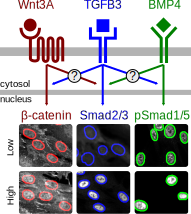
\includegraphics[width=3in]{FIGS/insulation/schematic.pdf}
  {\singlespacing 
  \caption[Schematic of the experimental system for \tgfbsf/Wnt crosstalk.]
        {Schematic of the experimental system for \tgfbsf/Wnt
         crosstalk. To measure inter-pathway signaling crosstalk,
         ligands can be applied combinatorially, followed
         by measurement of nuclear transcription
         factor levels. As shown, Wnt3A increases global
         quantities of \bcat, \tgf 3 causes translocation
         of bulk Smad2/3 to the nucleus, and levels of nuclear
         phospho-Smad1/5/8 increase upon BMP4 treatment.
         HCECs, with (``High'') or without (``Low'') 2hr treatment by
         Wnt3A (240ng/mL), \tgf 3 (4ng/mL), or BMP4 (73ng/mL).
         Outlines are of nuclei, segmented from the Hoechst channel
         (channel not shown) using the same threshold-segmentation method
         as in all imaging studies in this chapter.
         Fields are chosen to demonstrate visually obvious
         outcomes of signaling, though the diversity of responses
         is quite high for all pathways
         (see Figs. \ref{fig:insulation:ligandInformation} \&
         \ref{fig:insulation:readoutInformation}).}
  \label{fig:insulation:schematic}}
  \end{figure}
  

I reasoned that, because transcription factor activity is
the direct endpoint of signal transduction, I can infer the
degree of meaningful \tgfbsf\ and Wnt signaling interaction by measuring
how stimulation of one pathway affects the immediate transcription factor
response of the other pathway (\ar{fig:insulation:schematic}).
Current studies typically rely on transcriptional readouts to infer
such interactions, but these inferences may be confounded by transcriptional
feedback (which I consider to be the result of nuclear decision-making,
not signal transduction). Therefore, to accurately interpret cross-pathway effects
with respect to signaling, I use experimental timepoints that are
as close to the initial signaling event as possible.
Additionally, it is widely
believed that both Wnt and \tgfbsf\ signaling can be highly context-dependent.
I therefore repeat the experiments in this chapter using multiple
cell types, chosen to represent divergent cellular contexts.
By doing so, the hope is that any resulting shared properties of signal
integration can be more confidently extrapolated to other cellular systems.

In order to rigorously quantify single-cell responses to the
many experimental conditions required for this study,
and to make use of the expertise within the Altschuler \& Wu
lab, I use high-throughput immunofluorescence imaging as my primary
experimental platform. Unless otherwise indicated,
the presented measurements in this chapter originate from the
total-intensity feature values of individual nuclei. I typically report the
population-medians of these single-cell values, from replicate experimental
setups (as shown schematically
in \ar{insulation:system:measurement}; see \ar{imaging:introduction}
for more detail on my approach to image analysis).


  \begin{figure}[!bt]
  \centering
  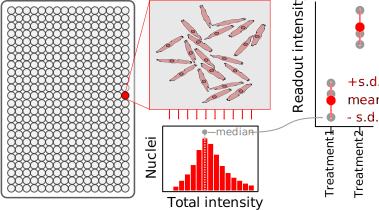
\includegraphics[width=3in]{FIGS/insulation/measurementSchematic.pdf}
  {\singlespacing 
  \caption[Schematic of the population-level fluorescence metric.]
        { 
        The fluorescence intensities reported in this
        chapter are population-level, based on single-nuclei
        measurements. As shown schematically here,
        cells are treated in
        96- or 384-well plates (left) and then fixed, immunostained,
        and imaged (middle, top).
        Nuclei are then identified computationally
        (see \ar{imaging:features}) so that the distributions
        of single-nuclei total fluorescence are obtained
        (middle, bottom). The medians of these distributions are
        then calculated for each replicate well. The reported
        values in this chapter are the means and standard deviations
        of these median values, nearly always from $n$=3 replicates.
        P-values are then calculated using an unpaired, two-tailed
        Student's t-test, and significant differences (p<0.05) are
        indicated with an asterisk. Figure legends indicate
        which samples are being compared for
        statistical significance.
        }
  \label{insulation:system:measurement}}
  \end{figure}
  

\subsection{Choosing cell types}
\label{insulation:system:readouts}


In order to choose useful cell lines, ligands, and readouts
for the study of Wnt and \tgfbsf\ signaling, I was confronted
with something of a chicken-or-the-egg problem. However, ongoing work
within the Altschuler \& Wu 
lab had made use of purified recombinant \tgf 1 for stimulating
the \tgf\ pathway and a total-Smad2/3 antibody for measuring the response.
Additional work had shown the efficacy of a \bcat\ antibody for
measuring cellular responses to purified Wnt3A. I therefore first made
use of these reagents, using literature-supported concentrations,
to identify cell lines that show responsiveness
to these pathways.


  \begin{figure}[!bt]
  \centering
  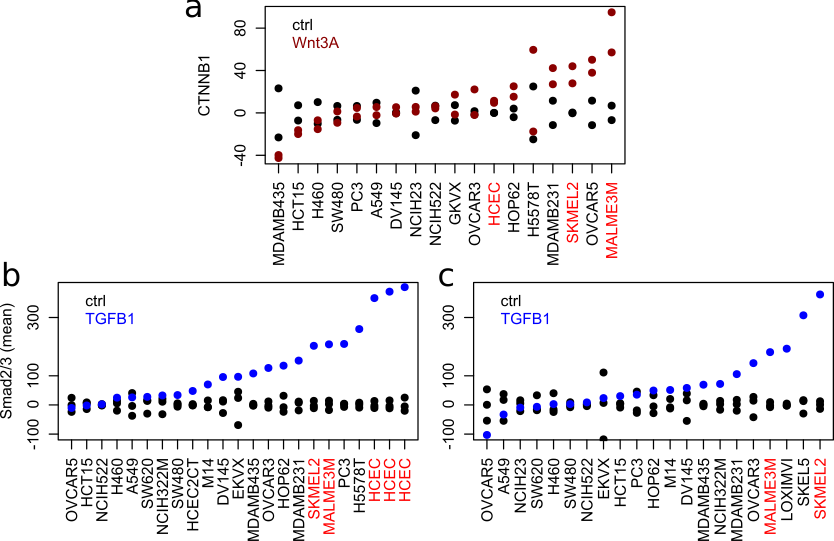
\includegraphics[width=6in]{FIGS/insulation/celltypeScreen.pdf}
  {\singlespacing 
  \caption[A screen for Wnt and \tgf\ responsive cell lines.]
        { A screen for Wnt3A (\b{a}) and
          \tgf 1-responsiveness (partial-replicate screens
          \b{b} and \b{c}) 
          across $\sim$20 cell lines revealed consistent
          responses by human colonic epithelial
          cells (HCECs) and two melanoma lines
          (SKMEL2 and MALME3M), highlighted with bright red text.
          The measured single-cell feature is the nuclear
          mean of fluorescence intensity by imaging
          (arbitrary units). Plots show the median
          of these single-cell values across all cells in
          a treated well (as in \ar{insulation:system:measurement}).
          The control means are subtracted from all values, per cell line,
          to show absolute changes in nuclear intensity.
          Concentrations: 1ng/mL \tgf 1, 200ng/mL Wnt3A.
          Timepoints: 1.25hrs (Wnt3A), 1hr (\tgf 1).
        }
  \label{fig:insulation:celltypeScreen}}
  \end{figure}


I first selected an immortalized (via telomerase and CDK4 expression)
but non-transformed human colonic epthelial cell (HCEC) line. This
cell line has stable ploidy and properties consistent with it being
a pseudo-differentiated cell type \cite{Roig2010}. Given the importance
of Wnt and \tgfbsf\ signaling in the gut (\ar{pathways:wntTgfb:gut}),
this cell line makes for a
reasonable model system for studying crosstalk between these pathways.
As a control, I also chose the rat small intestine
epithelial line (IEC6) \cite{Quaroni1978},
reasoning that it should display similar properties to HCECs.
I found that both of these
cell types respond strongly (in a statistical sense)
to TGFB ligands, moderately to BMP4,
and weakly (but measurably) to Wnt3A.


As discussed in \ar{introduction:encoding:context}, signaling
pathways generally show context-dependency, especially with respect
to differences in cell type. This non-generality is especially
true of the \tgfbsf\ and Wnt pathways (\ar{pathways:introduction}).
Therefore, in order to discover general properties (if indeed they exist)
we need to look for commonalities across cell types; the two intestinal
cell lines chosen may not be sufficient to infer generality. 
One approach to increase generality would be to
exhaustively test a large number of cell types, so that with each
successive cell type we gain confidence in the generality of a biological
phenomenon. Unfortunately, this approach is costly and difficult, and still
does not lead to certainty in the generality of a discovered phenomenon.
I opted then for a simpler approach, which is to test a small number of
divergent cell types. In this way, any behaviors consistent
across cell types can still be extrapolated as ``general'' behaviors,
though the resulting confidence in such a generalization may be somewhat
lower. 


To identify additional cell types for studying \tgfbsf\ and Wnt
crosstalk, I screened a panel of cancer cell lines for responsiveness
to \tgf 1 and Wnt3A. 
Additional selection criteria included cell morphology and
growth patterns that would allow for accurate image segmentation (see
\ar{imaging:features}), as well as cellular
growth rates and adherence properties that would
allow for the throughput needed for the many experimental conditions
required in my studies.
Two melanoma cell lines, SKMEL2 and MALME3M,
satisfied these criteria and were consistently ranked among the most
responsive to both \tgf 1 and Wnt3A (\ar{fig:insulation:celltypeScreen}).
Both of these cell lines can form malignant melanomas in nude mice, and
have abnormal ploidy  \cite{Fogh1977}. In particular, I found that SKMEL2 cells always
form tri-modal cell cycle distributions, implying the presence of diploid,
tetraploid, and octoploid cells within an asynchronous cycling population.
To my knowledge, there are no Wnt or \tgfbsf\ pathway mutations in SKMEL2
or MALME3M cells.


These cell lines should not be used to make
inferences with respect to differences between ``normal'' and cancer
cells, as these cell lines differ also in tissue of origin. Instead,
they should be thought of simply as divergent pairs of cell types that provide
consistent ``contexts'' (e.g. within the two intestinal lines or
within the two melanoma lines ) as well as divergent contexts (e.g.
between the intestinal and melanoma lines).
For all analyses in this chapter, I use only those cells
within the first peak of the imaging-based cell cycle distributions
(see \ar{imaging:variation:dnaQC}). I verified for each individual
pathway that the position of a cell within the cell cycle distribution
was not predictive of pathway behavior (data not shown) and
restriction to the G1/0 cell cycle phase otherwise reduces both experimental noise and
unimportant biological variation.
  
  
\subsection{Choosing signaling inputs and outputs}
\label{insulation:system:inputOutput}


Having chosen the cellular contexts in which to measure
the signaling crosstalk between \tgfbsf\ and Wnt, I then
needed to choose inputs and outputs that
could be believably interpreted to represent these pathways.
As discussed in \ar{introduction:encoding}, as a rule it
is not known what aspects of a signal or a readout are the
most relevant carriers of information for a cell. It is
generally believed, however, that for morphogenic pathways
it is the extracellular concentration of a ligand and the
nuclear concentration of a corresponding transcription factor that
are the relevant parameters. I therefore tested several ligands and readouts
in order to identify experimental inputs and outputs that are
both meaningful and practical.


  \begin{figure}[!bt]
  \centering
  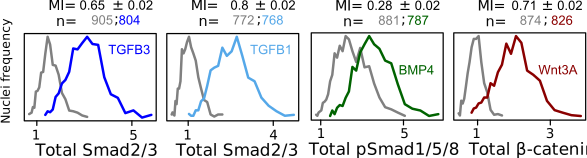
\includegraphics[width=6in]{FIGS/insulation/ligandInformation+.pdf}
  {\singlespacing 
  \caption[Information content of experimental treatments.]
        { Saturating ligand concentrations of \tgf 1/3 (12ng/mL), 
          Wnt3A (730ng/mL),
          and BMP4 (8ng/mL) are informative with respect to
          their canonical
          transcription factors. MI,
          mutual information between the ligand and readout
          (in bits, maximum MI is 1, see \ar{imaging:information}). 
          Histograms, distributions
          of single-cell total nuclear intensities for the
          immunostained transcription factors. $n$, number of cells
          per histogram, pooled from 3 replicate wells 
          (color-coded). Gray, untreated. 
          SKMEL2 cells, 1hr treatment. Arbitrary fluorescence units,
          frequencies scaled to have the same maximum value for display
          purposes.}
  \label{fig:insulation:ligandInformation}}
  \end{figure}
 
\subsubsection{Choosing prototypical ligands}
 
I first assayed several pathway inputs for information
content and signaling specificity. For the BMP2/4 pathway, I found that
all cell lines were non-responsive to purified BMP2 (data not shown) but
responsive to purified BMP4. These two ligands are
highly homologous and are thought to act through the same receptors
(\ar{pathways:tgfb:ligands}) therefore this absence of effective BMP2
signaling does not have a clear interpretation (perhaps a faulty reagent). In any event, the 
BMP4 signal is informative (using the mutual information metric,
as described in \ar{imaging:information});
the distribution of single-cell responses to saturating BMP4 is wide
but significantly different from the control distribution 
(\ar{fig:insulation:ligandInformation}). 


For the \tgf\ pathway I compared \tgf 1 and \tgf 3, as these ligands
are considered to be essentially interchangeable
(\ar{pathways:tgfb:ligands}). Indeed, within a single experiment
these two ligands generated similarly broad and separated Smad2/3
responses with similar mutual information
(\ar{fig:insulation:ligandInformation}). Dose-response curves for
the two ligands have the same
maxima and similar hill coefficients, though \tgf 3 is $\sim$10 time more
efficacious than \tgf 1 (data not shown).
\tgf 3 generally yielded more reliable responses, and so I use this
ligand for the remaining experiments in this chapter.


Finally, I chose to use purified Wnt3A to stimulate the canonical
Wnt pathway. Wnt3A is considered the prototypical ligand for this
pathway (\ar{pathways:wnt:wnt}), and its commercially-available
purified form has been widely used throughout the literature.
Importantly, I discovered that what is likely the most
commonly-used form, a low-purity ($\sim$75\%)
version from R\&D Biosystems, is sufficient to send Smad2/3 to the nucleus with the same
kinetics and dose-response Hill coefficicent as seen with \tgf\ treatment
(\ar{fig:insulation:contamination}a). I was unable to measure contaminating \tgf\ ligands
by Western (\ar{fig:insulation:contamination}b),
though this could be due to low concentrations of a high-efficacy \tgf\ variant.
In any event, this pathway crosstalk is likely
a consequence of trace amounts of contaminating \tgf\ in
the purified Wnt, as a pan \tgf-blocking antibody is sufficient to
block this response. Further, high-purity and carrier-free variants of the
product do not activate Smad2/3 (\ar{fig:insulation:contamination}c).


This artifactual crosstalk also occurs with the prototypical non-canonical
Wnt5A (\ar{fig:insulation:contamination}a,c), which casts
uncertainty onto recently-published work
linking Wnt5A and \tgf\ signaling
(reviewed in \ar{pathways:wntTgfb:dvl}) \cite{Miyoshi2012}.
The presence of such contamination may complicate the
interpretation of many other published studies, as it
suggests that treatment with purified Wnt3A or Wnt5A may generally include treatment
with \tgf, such that some resulting phenotypes 
could be due to stimulation by Wnt, \tgf,
or both.


  \begin{figure}[!bt]
  \centering
  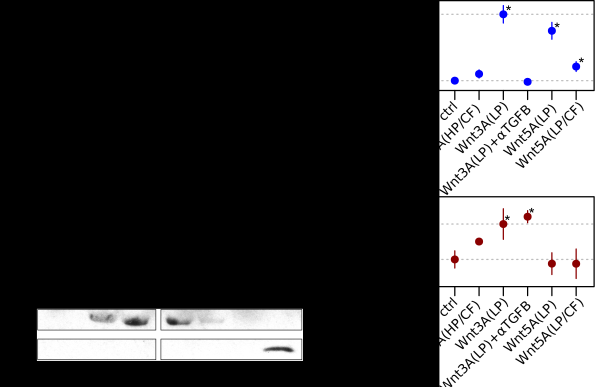
\includegraphics[width=5in]{FIGS/insulation/contamination+.pdf}
  {\singlespacing 
  \caption[Contamination of commonly-used commercial Wnt3A.]
        { The commonly-used low-purity (75\%) Wnt3A and Wnt5a ligands have
          trace amounts of contaminating \tgf.
          \b{a}, Dose-response curves
          for Wnt3A and Wnt5A against Smad2/3 yield EC$_{50}$ concentrations for
          the Wnts that are comparable to those used in the literature
          to stimulate Wnt responses (>100ng/mL is common).
          Duplicate experiments. Median of the mean nuclear
          intensity is plotted for each well (as in \ar{insulation:system:measurement}).
          \b{b}, Western blot of
          the purified Wnt3A ligands using a pan-\tgf\ antibody. HP/CF
          is the high-purity/carrier-free ligand used throughout this
          chapter, +BSA is the low-purity Wnt3A. BSA is shown as a reference.
          The low-purity Wnt3A lane should contain
          $\sim$25\textmu{g} of BSA in this blot, which is enough protein
          to soak up significant \tgf\ antibody.
          \tgf 1 is $\sim$12 kiloDaltons.
          \b{c}, The apparent Wnt$\rightarrow$Smad2/3 response is completely blocked
          by co-treatment with a pan-TGFB antibody that does
          not block the ability of Wnt3A to stimulate a \bcat\
          response. Low-purity Wnt5A also stimulates Smad2/3,
          but a carrier-free (CF) version does not. The high-purity (>90\%)
          carrier-free (HP/CF) Wnt3A shows a minimal Smad2/3
          response that is reproducible in other experiments, though not significant
          in this one. Concentrations: Wnt3A (200ng/mL),
          Wnt5A (100ng/mL), \textalpha{TGFB} (5\textmu{g}/mL).
          Y-axes and p-values as in 
          \ar{fig:insulation:specificity}.
          \b{a,c}, HCECs, 1hr treatment.}
  \label{fig:insulation:contamination}}
  \end{figure}

  
I therefore use high-purity/carrier-free Wnt3A for all experiments
in this chapter. I note, however, that even this ligand often causes
a small increase in Smad2/3 and so crosstalk experiments must be
interpreted with this fact in mind.

  
\subsubsection{Choosing prototypical readouts}


Having identified robust pathway inputs, I then needed to validate
antibody-based pathway outputs for immunofluorescence imaging.
For the \tgf\ pathway, which specifically activates Smad2/3,
and the BMP4 pathway, which specifically activates Smad1/5/8
(see \ar{pathways:tgfb:smads}),
I find that the nuclear fractions of both active phospho-protein and
total-protein levels can respond robustly to pathway activation.
However, it is unclear from the literature whether it is the total
concentration or the phospho-state concentration that encodes
extracellular ligand levels.


  \begin{figure}[!bt]
  \centering
  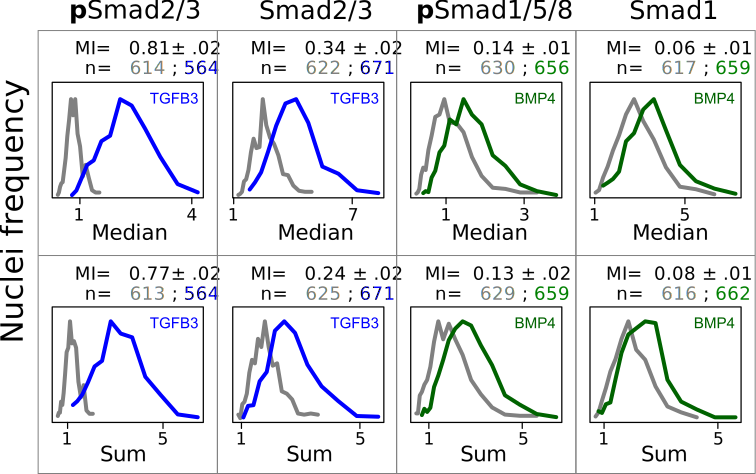
\includegraphics[width=5.5in]{FIGS/insulation/readoutInformation+.pdf}
  {\singlespacing 
  \caption[Information content of Smad readouts.]
        { Nuclear phospho-Smads (pSmads) contain more information about
          ligand concentrations than do nuclear total-Smads,
          though the sum and mean of intensity features are comparable. The
          untreated (gray) and treated (colored) distributions
          of single-nuclei measurements show more overlap
          of total-Smad readouts, resulting in relatively less mutual
          information (MI, in bits, maximum of 1, see \ar{imaging:information}).
          The median (top row) and
          sum (bottom row) of nuclear intensities for a single readout
          have nearly identical information content.
          $n$, number of cells
          per histogram (color-coded). 
          Ligand concentrations: saturating 10ng/mL
          \tgf 3 (blue) or 50ng/mL BMP4 (green).
          SKMEL2 cells, 1.5hr treatment. Arbitrary fluorescence units,
          frequncies normalized to have same maximum value.}
  \label{fig:insulation:readoutInformation}}
  \end{figure}


I therefore measured the mutual information
between these readouts and their ligands, which
revealed that the phospho-state is indeed more informative
(\ar{fig:insulation:readoutInformation}). Care should be taken when
interpreting this data, however, as the difference in information content
may also be due to antibody specificities, along with a myriad of
other causes. I note that
I have never observed maximum mutual information values of more than $\sim$1.2 bits
for any type of input/output relationship from imaging data, consistent
with published reports \cite{Cheong2011}.
The most fair statement, then, is that these particular approximations
of the phospho-state are more informative than these approximations of
total protein levels.


The total-Smad2/3 antibody yielded more-consistent
results across experiments than did the phospho-Smad2/3 antibody,
however, and has similarly-high
information content. I therefore use the total-Smad2/3
and the phospho-Smad1/5/8 (pSmad1/5/8) antibodies for the crosstalk experiments.
For canonical Wnt signaling there is strong evidence that it is the
total-protein level of \bcat, not the phospho-state, that encodes ligand concentration
(\ar{pathways:wnt:bcat}). I therefore use a total-protein \bcat\ antibody
to measure canonical Wnt responses.


\subsubsection{Validating input/output relationships}



  \begin{figure}[!bt]
  \centering
  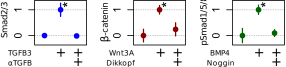
\includegraphics[width=4.5in]{FIGS/insulation/specificity+.pdf}
  {\singlespacing 
  \caption[Specificity of ligand/transcription factor relationships.]
        { The measured canonical transcription factor responses are a specific
          consequence of ligand treatment. \b{Left}, A
          pan-TGFB antibody (\textalpha{TGFB})
          blocks 2hr \tgf 3-induced
          nuclear Smad2/3 accumulation in HCECs. \b{Middle},
          Dikkopf, a soluble antagonist (\ar{pathways:wnt:frizzled}),
          blocks \bcat\ accumulation due to 2hr Wnt3A in
          SKMEL2s. \b{Right},
          Noggin, a soluble antagonist (\ar{pathways:tgfb:ligands}),
          blocks 1.5hr BMP4-induced phospho-Smad1/5/8 in SKMEL2s. Y-axes,
          median across single-cell nuclear intensities (the total feature)
          within a well. As in \ar{fig:insulation:schematic},
          points are the mean and standard deviation
          of $n=3$ replicate wells and `*' indicates one-sided p-value <0.05
          (Student's t-test) compared to control. Intensities normalized by
          $R_\text{i,norm}=\frac{R_\text{i}-\text{mean}(R_\text{ctrl})}
          {R_\text{ligand}-\text{mean}(R_\text{ctrl})}$.
          Concentrations: \tgf 3 (10ng/mL),
          \textalpha{TGFB} (5\textmu{g}/mL),
          Wnt3A (200ng/mL), Dikkopf (1\textmu{g}/mL),
          BMP4 (50ng/mL), Noggin (100ng/mL).}
  \label{fig:insulation:specificity}}
  \end{figure}
  
  
Aside from measuring the mutual information between each
input and output it is essential to ensure that
the input/output relationships are not artifactual. To do so, I verified
that each output could be blocked by a highly specific antagonist
\arp{fig:insulation:specificity}. 
Additionally, while I am primarily
interested in the signal transduction process, it is important
to ensure that a transduced signal leads to a nuclear decision.
In the case of \tgfbsf\ and Wnt signaling, this decision is
a change to the transcriptional network. The conserved
target for Wnt3A is Axin2, a negative auto-regulator
(\ar{pathways:wnt:bcat}). For \tgfbsf,
the conserved targets are the inhibitory-Smads (iSmads), Smad6/7
(\ar{pathways:tgfb:smads}). I therefore measured
mRNA levels of these transcriptional targets,
finding that stimulation does indeed yield transcription
in all cases (\ar{fig:insulation:expression}).


  \begin{figure}[!bt]
  \centering
  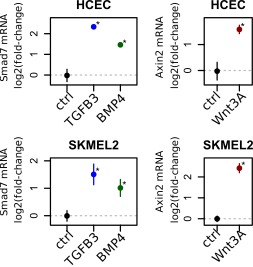
\includegraphics[width=3in]{FIGS/insulation/expression+.pdf}
  {\singlespacing 
  \caption[\tgfbsf\ and Wnt cause canonical target gene expression.]
        { The \tgf 3, Wnt3A, and BMP4 ligands cause
          expression of canonical target genes in the cell lines
          used in this dissertation. Fold-change
          is relative to the control condition. 2hr treatment. Concentrations:
          10ng/mL \tgf 3, 25ng/mL BMP4, 200ng/mL Wnt3A.
          Mean and standard deviation
          of 3 replicates, `*' indicates two-sided p-value <0.05
          (Student's t-test). mRNA levels measured by TaqMan qPCR
          (see \nameref{insulation:methods} for experimental details).
        }
  \label{fig:insulation:expression}}
  \end{figure}
  
 

  
  
\subsection{Interpretation of single-cell immunofluorescence measurements}


As for any method of measurement, it is important to
take a step back and think carefully about the biological
interpretation of the resulting data. For the image-based
single-cell data obtained in my work, cellular nuclei are
identified using Hoechst-staining and threshold segmentation,
and I only analyze those nuclei that likely belong to the G1 cell
cycle phase (see \ar{imaging:segmentation}).
Within these nuclei I tally up all pixel values to obtain
the total intensity feature, which I use as a proxy for
the quantity of the immuno-labeled target protein within the nucleus.
This feature and the mean intensity feature,
which is a proxy for concentration, are similarly informative
in my assays (\ar{fig:insulation:readoutInformation}), and
so I use the total-intensity feature for the practical
reasons described in \ar{imaging:totalIntensity}.
  

How do we interpret changes in this feature? Fold-change
over a reference (e.g. the untreated state) is a commonly used
metric, but the interpretation of fold-change is unclear in cases where
either the basal state is near zero (as any fold-change
value will move towards infinity) or is non-zero because of ``background'' signal
(which pushes all fold-change values towards 1). Using the
fluorescence image model that I present in 
\ar{imaging:model}, we can model the total intensity feature $T$
for any given nucleus $n$ by \ar{eq:system:total}. In this model the intensity of
each pixel $p$ is the sum of multiple fluorescence sources, such as
non-specific fluorescence ($F_{\text{nonspecific,}p}$,
e.g. due to off-target antibody
binding), non-signaling fluorescence ($F_{\text{nonsignaling,}p}$, 
e.g. due to a pool of the target
protein that is not involved in the studied signaling process), and the
actual signaling fluorescence $F_{\text{signaling,}p}$.
    %
    \begin{equation} \label{eq:system:total}
    T_n=\sum_p\left(F_{\text{nonspecific,}p}+F_{\text{nonsignaling,}p}+F_{\text{signaling,}p}\right)
    \end{equation}


Take the case of \bcat\ as an example. Basal
\bcat\ levels within Wnt3A-unstimulated cells are thought to be
essentially zero \arp{pathways:wnt:bcat}, and yet the measured basal levels are
quite high. This is due in large part to the presence of a
membrane-associated \bcat\ pool that does not participate in
Wnt signaling. It is impossible to know how the total nuclear
intensity breaks down into the various components of
\ar{eq:system:total}, and therefore
a metric like fold-change is uninterpretable in terms of the extent
of change for \bcat, though it can be used as a normalization method
to allow for measurements of relative change.


An alternative metric is to simply subtract a reference intensity measurement
from the experimental intensity, as the only term remaining will
be $F_\text{signaling,experiment}-F_\text{signaling,ctrl}$.
While this metric has a simple interpretation (absolute change in
signaling-associated fluorescence intensity), unfortunately it cannot be
used to infer the absolute magnitude
of response since fluorescence units are arbitrary.
Neither division nore subtraction can be used at the
single-cell level for fixed-cell assays,
as the relative contribution of each fluorescent component may vary
from cell to cell. Both metrics can be used
at the population level, however.


In summary, it is impossible to infer the absolute magnitude of change for
a signaling molecule using image-based immunofluorescence without
making assumptions that would be indefensible for the
immunofluoresce studies in this chapter. External
means of validation are then required to show that the observed
change is large enough to have a meaningful effect (as in
\ar{fig:insulation:expression}, where I show that the same experimental
treatments yield sizeable changes to target gene expression).
Relative comparisons between experimental perturbations are possible in any case,
and are easy to understand,
and so for convenience I use units normalized to a 0/1 scale throughout this chapter.


\subsection{Timepoints and concentrations}


Many studies of morphogenic signaling
pathways conflate the signal transduction and the transcriptional
decision-making processes due to use of long-term transcriptional
readouts. This conflation may be acceptable for some experimental
questions, but here my aim is to study integration specifically at
the level of signal transduction.


  \begin{figure}[!bt]
  \centering
  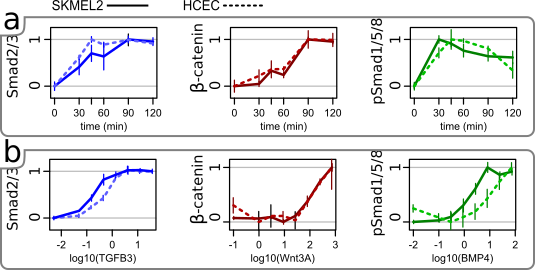
\includegraphics[width=6in]{FIGS/insulation/doseTime.pdf}
  {\singlespacing 
  \caption[Dose-response and timecourse of \tgfbsf\ and Wnt.]
        { The cell lines tested in this dissertation have similar
          but non-identical timelines (\b{a}) and
          dose-response curves (\b{b}). Shown
          are SKMEL2 (solid lines) and HCEC (dashed lines) cell lines.
          Cell lines show measurable responses between 60-120 minutes
          and are saturated by 10ng/mL \tgf 3, 1000ng/mL Wnt3A,
          or 100ng BMP4. Dose-responses are at 1hr.
          Y-axes as in \ar{fig:insulation:specificity},
          normalized so that the minimum and maximum responses
          are 0 and 1. Concentrations used in \b{a}:
		  TGFB3 (4ng/mL), Wnt3A (240ng/mL), BMP4 (70ng/mL).}
  \label{fig:insulation:doseTime}}
  \end{figure}
  

To do so, it is then necessary to minimize the effects of transcriptional
feedback on the stimulated pathways. I therefore performed
time-course experiments for each cell line and pathway in order to identify the
earliest timepoints that could still yield robust pathway responses
(shown for HCEC and SKMEL2 in \ar{fig:insulation:doseTime}a). For
all cell lines and pathways the responses were measurable by 1hr and
maximal by 2hrs, and so my crosstalk experiments take place within
this temporal window.
  

As I discuss in \ar{introduction:encodingSolution}, it is not necessarily true
that the use of a constant ligand concentration across multiple cell lines
is the appropriate way to ensure that the treatment is the ``same.'' Fortunately,
the dose-response curves for each cell line and pathway are not wildly different
(shown for HCEC and SKMEL2 in \ar{fig:insulation:doseTime}b) and so I was able
to determine concentrations that would yield approximately half-maximal responses (EC50)
or maximal responses across all cell types.


The reader may notice the use of differing ligand concentrations between
the experiments in this chapter.
For initial experiments, I did not yet know how responsive the cell types were
to each ligand, and so concentrations were based on prior work in the lab or
on literature-obtained values. For later experiments, doses were first chosen
according to whether a half-maximal or maximal response was experimentally
required, and these doses were then kept high over time to maintain saturating
levels in the face of slowly-degrading reagents and idiosyncratic sensitivities
of cell lines. Importantly, saturating concentrations
minimize the consequences of pipetting
error, since larger error can be tolerated before a measurable difference
in cellular responses will appear.



\section{Signaling integration between Wnt and \tgfbsf}
\label{insulation:wntTgfb}

Up to this point, the content of this dissertation has
all been designed to set up the question: To what extent
do Wnt and \tgfbsf\ interact during signal transduction,
prior to nuclear entry? As discussed throughout
\ar{pathways:introduction}, these pathways have extensive
opportunity for interaction and are widely believed to
integrate information at the level of transcription. Further,
despite a lack of shared core components, these signaling
pathways have been tied together by numerous studies
showing cross-pathway protein-protein
interactions \arp{pathways:wntTgfb:mechanism}. What is still unclear,
however, is whether these interactions take place and have
functional consequences to signal transduction under endogenous levels of
pathway components.


\subsection{Wnt3A and \tgf 3 show complete signaling insulation}


To measure the signaling crosstalk between \tgf\ and canonical
Wnt,
I made use of the experimental strategy described in the previous
section by treating cells with combinations of each ligand.
If these pathways
were to interact in a manner that affects signaling (i.e.
in a manner that transfers information) then
the direct outcome of signaling (that is, nuclear canonical
transcription factor levels) would be affected.


  \begin{figure}[!bt]
  \centering
  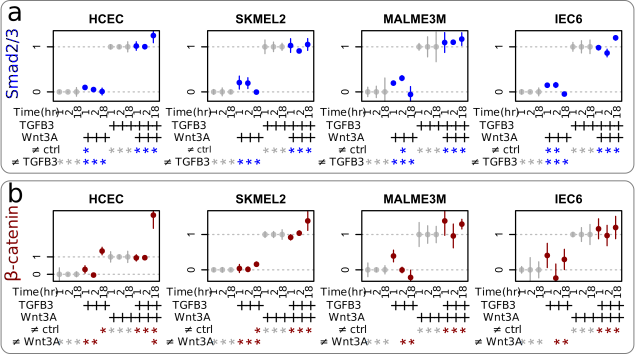
\includegraphics[width=6.5in]{FIGS/insulation/wntTgfbInsulation+.pdf}
  {\singlespacing 
  \caption[Wnt and \tgf\ are insulated during signal transduction (all data).]
        { Wnt and \tgf\ are insulated during signal transduction.
          \b{a}, Wnt3A causes little or no modulation of Smad2/3 responses at
          both short (1-2hr) and long (18hr) timepoints for all
          cell lines tested. \b{b}, \tgf 3 causes little or no
          modulation of \bcat\ responses, except in the case of
          long-term treatment in HCECs (note the 18hr \tgf 3 and 
          \tgf 3+Wnt3A responses). Y-axes and p-values as in
          \ar{fig:insulation:specificity}, with normalization per
          timepoint to set the control to 0 and the canonical-input-only
          condition to 1. These values fixed by normalization are in gray.
          $n=3$ replicates per point. p-values indicate
          whether each condition differs from control
          ($\neq$ctrl) or from the canonical-input-only
          condition (either $\neq$\tgf 3 or $\neq$Wnt3A).
          Concentrations (1 and 2hr): 0.2ng/mL \tgf 3,
          100ng/mL Wnt3A. Concentrations (18hr): 10ng/mL \tgf 3,
          200ng/mL Wnt3A.
          }
  \label{fig:insulation:wntTgfbInsulation}}
  \end{figure}
  

  \begin{figure}[!bt]
  \centering
  \includegraphics[width=5in]{FIGS/insulation/wntTgfb_summary.pdf}
  {\singlespacing 
  \caption[Wnt and \tgf\ are insulated during signal transduction (summary).]
        { Summary figure for insulation between Wnt3A and \tgf 3,
          limited to SKMEL2s and HCECs at 2 and 18hrs.
          \b{a}, At 2hrs, there is complete signaling insulation between
          Wnt3A and \tgf 3.
          \b{b}, However, context-dependent transcriptional integration
          already occurs at the same timepoint: HCECs show inhibition of
          Axin2 mRNA expression by \tgf 3 treatment, while SKMEL2s show
          complete transcriptional insulation.
          \b{c}, This context-dependent effect shows up at the level
          of signaling hours later, in HCECs. The increase in \bcat\ due
          to \tgf 3 signaling likely stems from the inhibition of Axin2
          mRNA (since Axin2 is a negative auto-regulator of Wnt3A). Thus,
          signaling insulation (\b{a}) combined with transcriptional integration
          (\b{b}) leads to a new, biased signaling state over time (\b{c}).
          Daggers
          indicate significant departure from pathway insulation.
          Data for \b{a} and \b{c} from \ar{fig:insulation:wntTgfbInsulation}.
          Data for \b{b} from \ar{fig:insulation:expressionXtalk}.
          }
  \label{fig:insulation:wntTgfbSummary}}
  \end{figure}
    

  
To test this, I treated all four cell types with combinatorial
inputs of \tgf 3 and Wnt3A, and then measured nuclear accumulation
of the transcription factors Smad2/3 and \bcat\ by
single-cell image analysis.
Data for all four cell lines are shown for 1, 2, and 18hr timepoints in
\arp{fig:insulation:wntTgfbInsulation}. This is a lot of data, and so
for simplicity I refer the reader to \ar{fig:insulation:wntTgfbSummary}, which shows
only the essential data for HCECs and SKMEL2s.


I performed the initial experiment at 1 and 2hr timepoints, using
ligand concentrations that ranged from EC50 to saturating across
the cell lines. In all cases, Wnt3A had small or
statistically insignificant effects on Smad2/3 levels, even when 
co-treated with \tgf 3 (\ar{fig:insulation:wntTgfbInsulation}a,
1 and 2hr timepoints; \ar{fig:insulation:wntTgfbSummary}a, top).
The small Wnt3A-induced Smad2/3 increases may be
real, but are likely due to the trace contamination discussed earlier
(see \ar{fig:insulation:contamination}). 
The same absence of signaling integration occurs in the other direction,
from \tgf 3 to \bcat\ (\ar{fig:insulation:wntTgfbInsulation}b,
1 and 2hr timepoints; \ar{fig:insulation:wntTgfbSummary}a, middle).
In this case, the presence of \tgf 3 had no significant effects
on \bcat\ levels in any context. Therefore, Wnt3A and \tgf 3 
are completely insulated during signal transduction
(\ar{fig:insulation:wntTgfbSummary}a, bottom).


Because the literature is full of examples of these two pathways interacting
over longer timescales, I decided to repeat the experiment with a more distant
timepoint.
To ensure that the absence of crosstalk was not due to low activity of the
pathways.
To my surprise, even at 18 hours there was almost no measurable modulation
of the transcription factor activity of one pathway by the other
(\ar{fig:insulation:wntTgfbInsulation}, 18hrs). There was
one exception, however: HCECs show \tgf 3$\rightarrow$\bcat\ interaction
(\ar{fig:insulation:wntTgfbSummary}c, middle). Indeed,
\tgf 3 treatment alone was sufficient to activate \bcat, and co-treatment
with Wnt3A yielded an approximately additive effect.


The complete absence of cross-pathway transcription factor modulation
at early timepoints strongly suggests that the Wnt3A and \tgf 3
signaling cascades are completely insulated from one another,
displaying no signaling crosstalk whatsoever
(\ar{fig:insulation:wntTgfbSummary}a, bottom). Further,
the frequent absence of cross-pathway modulation even given significant
time for transcriptional feedback shows that pathway insulation can be
maintained even after the transcriptional network has been remodeled by
morphogenic signals. Finally, the fact that HCECs lose this insulation
at later timepoints demonstrates a case of context-dependency
(i.e. dependency on cell type) in cellular decision-making
despite context-independent insulation of signal transduction
(\ar{fig:insulation:wntTgfbSummary}c, bottom).

  
\subsection{Wnt and \tgfbsf\ show context-dependent transcriptional integration}
 

Due to the surprising result that the direct outcomes of signaling
(transcription factor levels) are completely insulated between Wnt3A and \tgf 3,
I decided to test for insulation at the level of transcription. By
measuring mRNA expression 2hrs after treatment, I reasoned that I could
identify whether insulation at the level of signaling (as
already demonstrated) necessarily
implies insulation at the level of transcription. Because Axin2 and
Smad6/7 are the only prototypical transcription targets of the \tgfbsf\
and Wnt pathways, I measured mRNA levels of these genes following
combinatorial ligand treatment (\ar{fig:insulation:expressionXtalk};
simplified in \ar{fig:insulation:wntTgfbSummary}b).
 
 
  \begin{figure}[!bt]
  \centering
  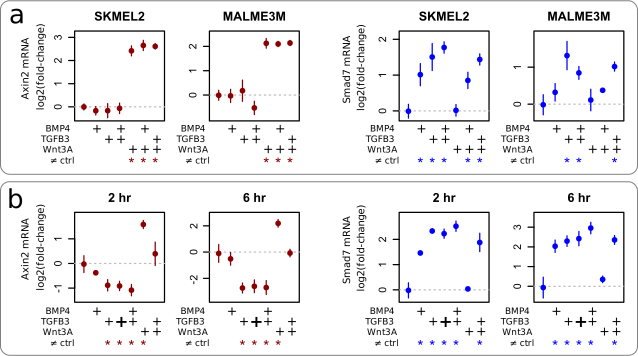
\includegraphics[width=6in]{FIGS/insulation/expressionXtalk.pdf}
  {\singlespacing 
  \caption[ Wnt and TGFB show context-dependent transcriptional crosstalk.]
        { Wnt and TGFB show context-dependent transcriptional crosstalk.
          \b{a}, In the melanoma cell lines, \tgf 3/BMP4 have no effect on
          Axin2 expression, while Wnt3A treatment has no effect on
          Smad7 expression. 2hr treatment.
          \b{b}, In HCECs, \tgf 3 reduces baseline and blocks
          Wnt3A-induced Axin2 expression. This effect is already apparent
          at 2hrs and is maintained at 6hrs. Wnt3A does not affect
          Smad7 expression in any context. Bold `+' indicates doubled
          \tgf 3 concentration, demonstrating transcriptional saturation of this pathway.
          Fold-change is relative to the control condition.
          Mean and standard deviation
          of 3 replicates, `*' indicates two-tailed p-value <0.05
          (Student's t-test).
          Concentrations: 10ng/mL \tgf 3, 25ng/mL BMP4, 200ng/mL Wnt3A.
          See \nameref{insulation:methods} for qPCR details.
        }
  \label{fig:insulation:expressionXtalk}}
  \end{figure}
  

By qPCR, neither of the melanoma cell lines show transcriptional
crosstalk between the canonical \tgfbsf\
and Wnt3A outputs Smad7 and Axin2
(\ar{fig:insulation:expressionXtalk}a), implying that these pathways
are insulated both in terms of the quantity of the transcription factors
sent to the nucleus (as shown in \ar{fig:insulation:wntTgfbInsulation})
and in the general activity of those
transcription factors. (This is not to say that these transcription factors
do not affect one another for any transcriptional targets.)
However, as before, HCECs display a different behavior.
By 2 hours HCECs show strong modulation of Axin2 expression
by \tgf 3 treatment(\ar{fig:insulation:wntTgfbSummary}b),
and this effect increases over time
(\ar{fig:insulation:expressionXtalk}b).


The modulation of Axin2 by \tgf 3 in HCECs is intriguing for
several reasons. First, it provides a simple explanation for the
18hr transcription factor modulation result observed in
(\ar{fig:insulation:wntTgfbSummary}c), since repression of Axin2,
a negative autoregulator of \bcat, could block the negative feedback
otherwise present after Wnt3A stimulation. Second, it clearly
shows that HCECs can simultaneously display signaling insulation
and transcriptional crosstalk,
demonstrating that these two processes can be completely
independent. Finally, the general lack of crosstalk across all
cell lines, coupled with the single instance of transcriptional
crosstalk in HCECs, is suggestive that the oft-cited idiosyncratic
outcomes of Wnt/\tgfbsf\ crosstalk are predominantly due to
context-dependent transcriptional crosstalk.



\section{Signaling insulation between BMP and \tgf}
\label{insulation:bmpTgfb}


 
  \begin{figure}[!bt]
  \centering
  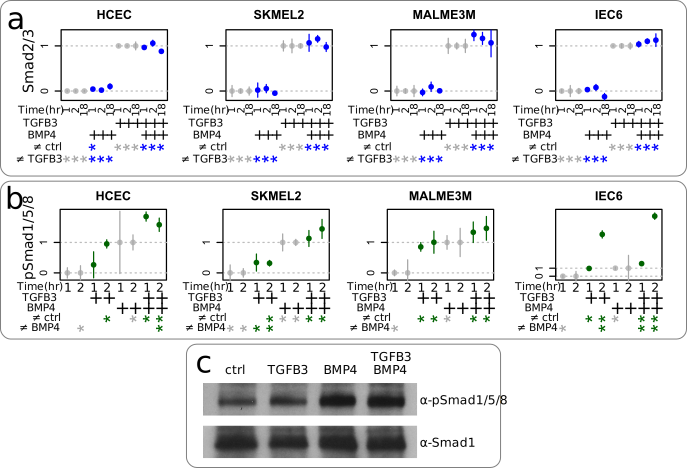
\includegraphics[width=6.5in]{FIGS/insulation/bmpTgfbInsulation.pdf}
  {\singlespacing 
  \caption[BMP4 and \tgf\ do not compete for Smad4 (all data).]
        { The \tgf\ and BMP signaling pathways are additive,
          and do not compete for Smad4. \b{a}, BMP4 causes no
          modulation of Smad2/3 responses at
          both short (1-2hr) and long (18hr) timepoints across all
          cell lines tested. \b{b}, \tgf 3 additively modulates pSmad1/5/8
          responses to BMP4. \b{c}, Measurement of \tgf 3/BMP4 crosstalk by
          Western is consistent with the imaging data. SKMEL2, 2hr treatment.
          \b{a,b}, Y-axes, normalization, and
          p-values as in \ar{fig:insulation:wntTgfbInsulation}. 
          Concentrations (1 and 2hr): 0.2ng/mL \tgf 3, 5ng/mL BMP4. Concentrations (18hr): 10ng/mL \tgf 3, 25ng/mL BMP4.
          Western courtesy Curtis A. Thorne (Altschuler \& Wu lab, UT
          Southwestern).
          }
  \label{fig:insulation:bmpTgfbInsulation}}
  \end{figure}



The above result is perhaps not so surprising,
that two pathways (Wnt3A and \tgf 3) lacking any shared core components do
not modulate one another during signal transduction. 
Under this rationale the BMP2/4 and \tgf 1/3 pathways
might then be expected to interact, given their shared requirement
for Smad4. Indeed, the claim of intra-\tgfbsf\ crosstalk 
via Smad4 competition has been cited in many reviews and papers,
but to my knowledge has not been directly tested
(\ar{pathways:tgfb:crosstalk}). I therefore
decided to use the same experimental setup as above to measure
the extent of crosstalk between BMP4 and \tgf 3
(\ar{fig:insulation:bmpTgfbInsulation}). The essential data is
again summarized in a simpler figure
(\ar{fig:insulation:bmpTgfbSummary}). If these pathways do 
compete for Smad4, then co-treatment with saturating concentrations
of both ligands (to maximize sequestration of Smad4) should cause one or
both pathways to be attenuated.

  \begin{figure}[!bt]
  \centering
  \includegraphics[width=5in]{FIGS/insulation/bmpTgfb_summary.pdf}
  {\singlespacing 
  \caption[BMP4 and \tgf\ do not compete for Smad4 (summary).]
        { Summary figure showing the lack of Smad4 competition between BMP4 and \tgf 3,
          limited to SKMEL2s and HCECs at 2hrs.
          \b{a}, There is additive signaling crosstalk from \tgf 3 to
          pSmad1/5/8, but not from BMP4 to Smad2/3.
          \b{b}, At the same time, the transcriptional output from the combined
          pathways also appears to be additive.
          \b{c}, Smad4 RNAi reduces protein levels of Smad4 in HCECs.
          Histone H3B serves as a loading control. 
          \b{d}, Smad4 RNAi in HCECs reduces overall \tgf 3 responsiveness (top)
          but not pSmad1/5/8 responsiveness (middle), while the signaling
          crosstalk between \tgf 3 and BMP4 remains approximately
          additive. Thus, competition for Smad4 does not cause cross-pathway
          signaling inhibition between \tgf 3 and BMP4. Normalization
          for \b{d} uses the control and single-ligand responses from
          the scramble siRNA treatment to define 0 and 1.
          Y-axes, normalization, and
          p-values as in \ar{fig:insulation:wntTgfbInsulation}. Daggers
          indicate significant departure from pathway insulation.
          Data for \b{a} from \ar{fig:insulation:bmpTgfbInsulation}.
          Data for \b{b} from \ar{fig:insulation:expressionXtalk}.
          Western courtesy Curtis A. Thorne (Altschuler \& Wu lab, UT
          Southwestern).
          }
  \label{fig:insulation:bmpTgfbSummary}}
  \end{figure}
    
  
  
BMP4 treatment
had absolutely no effect on Smad2/3 in any cell line
(\ar{fig:insulation:bmpTgfbInsulation}a;
 \ar{fig:insulation:bmpTgfbSummary}a,top). There is crosstalk
in the other direction:
treatment by \tgf 3 is sufficient to activate pSmad1/5/8, and
the presence of both ligands yields an additive behavior
(\ar{fig:insulation:bmpTgfbInsulation}b). Importantly, these
two pathways also have an approximately-additive effect on
transcription of their shared downstream target, Smad7
(\ar{fig:insulation:expressionXtalk}; \ar{fig:insulation:bmpTgfbSummary}b,top).
As noted
in \ar{pathways:tgfb:smads}, while the BMP2/4 and \tgf\ pathways
are generally considered to be distinct, they have been shown to
cross-activate one another in various settings.
Western blotting was not quantitative enough to confirm the
activation of pSmad1/5/8 by \tgf 3, but is consistent with an
absence of negative cross-regulation
(\ar{fig:insulation:bmpTgfbInsulation}c). In any case,
both the insulation of Smad2/3 from BMP4 and the additive
crosstalk between \tgf 3 and pSmad1/5/8 directly argue against
competitive inhibition between these pathways
during signal transduction.


I then wondered if the absence of inhibitory crosstalk
between BMP4 and \tgf 3 was a context-dependent phenomenon.
For example, the additive behavior is consistent
with the quantity of Smad4 being so high
as to be non-limiting, in which case both pathways would effectively have
distinct pools of Smad4 (as in \ar{fig:insulation:crosstalk}c).
I therefore used siRNA to knock down Smad4 in order to make Smad4 a
limiting factor in an effort to modulate the form of crosstalk
(e.g. to a non-additive form as in \ar{fig:insulation:crosstalk}d).


As a consequence of Smad4 depletion
(\ar{fig:insulation:bmpTgfbSummary}c), \tgf 3 signaling was strongly reduced overall
but was still not inhibited by co-treatment with BMP4
(\ar{fig:insulation:bmpTgfbSummary}d, top). Levels of pSmad1/5/8,
on the other hand, were not affected overall by Smad4 knockdown
(\ar{fig:insulation:crosstalk}d, top) and the effect of co-treatment
remained roughly additive. Therefore, in contrast to expectations,
BMP4 and \tgf 3 do not negatively regulate one another at all
at the level of signal transduction, and do
not compete for Smad4.



\section{Discussion}
\label{insulation:discussion}


In this chapter I measured the extent of crosstalk
between key morphogenic pathways, using a mechanism-independent
and endogenous approach that kept signaling crosstalk separable
from transcriptional crosstalk.
By doing so, I discovered that canonical Wnt and \tgf\
do not crosstalk at all during signal transduction, and that
\tgf\ and BMP do not compete for Smad4 during signaling.
Both of these results yield important simplifications to
the ever-increasing apparent complexity of signal transduction
that stems from discoveries of putative nodes of crosstalk.
Below, I discuss specific implications in more detail.


\subsection{Morphogenic signaling is insulated}


As I explain in \ar{pathways:discussion}, crosstalk during
signal transduction is likely to decrease the accuracy of the
intra-nuclear model of the extracellular environment. In such
a case, the information that eventually passes to the nucleus
for transcriptional processing represents a simplified view
of the cellular microenvironment, such that the nucleus then
has to make a decision with more uncertainty about the state of the outside world.
By instead allowing information to pass relatively unfiltered
from the extracellular milieu to the nucleus (e.g. by insulating
information channels from one another) the nucleus has access to a more
accurate model of the microenvironment and, presumably,
can then make more useful decisions.


The results presented in this chapter suggest that
the morphogenic Wnt and \tgfbsf\ pathways are indeed isolated
from one another, such that they can each pass information to
the nucleus without cross-pathway interference. As each pathway is only
capable of sending a small amount of information regarding
ligand concentration (not shown, but one can infer this from the broad distributions in Figs.
\ref{fig:insulation:readoutInformation} \&
\ref{fig:insulation:ligandInformation}), maintaining this
information from distinct pathways may be the only way
that a cell can obtain an accurate internal model of its
environment. Therefore, I propose that signaling insulation
may be a general property of morphogenic pathways whose
key outputs are changes to the transcriptional network.


Signaling insulation allows for the internalization of a
somewhat unfiltered view of the cellular microenvironment
(\ar{fig:insulation:wntTgfbSummary}a, cartoon).
Context-dependent transcriptional feedback
(\ar{fig:insulation:wntTgfbSummary}b, cartoon) can then modulate
the signaling pathways over time (either by auto-regulation or
cross-pathway regulation)
(\ar{fig:insulation:wntTgfbSummary}c, cartoon). The result of this nuclear
decision-making would be to essentially bias the
cell's view of what could even be an unchanging environment. Thus,
by mixing insulated signaling with long-term feedback,
cells can maintain a relatively complete internal model
of the environment but interpret that environment in a
temporally biased manner.


An obvious argument against general morphogenic insulation
in my own data is that \tgf 3 appears
to activate the BMP-specific Smads (Smad1/5/8). I note that
I was unable to verify that this crosstalk is specific (i.e.
not due to a contaminant) as addition of an anti-\tgf\
antibody along with \tgf 3 treatment did not significantly block
the interaction (data not shown). For this reason, I only
interpret the BMP/\tgf\ crosstalk data to say that one does not
inhibit the other.


An additional counter-argument is that these pathways
may in fact interact, but I have measured the wrong
thing to be able to identify the interactions. This would
be a useful discovery, as what my work shows is that
the generally-accepted method of encoding used by these
pathways shows complete insulation. It seems to me quite
possible that there exists some information channel, at
the level of signaling, that does indeed integrate information
from both Wnt and \tgf\ signals.


\subsection{BMP and \tgf\ do not compete for Smad4}


While it is widely believed that co-activation of the
BMP and \tgf\ pathways should result in some sort of
cross-pathway inhibition via Smad4 competition, I find
no evidence of this phenomenon. Indeed, I am unaware
of any studies that explicitly show this form of crosstalk,
and some studies have shown that Smad4 is highly
abundant \cite{Nicolas2004,Clarke2006}.


Interestingly, my data show that even when Smad4
is brought down to limiting levels, there is still no
cross-pathway inhibition. Smad4 is seen as
the factor that allows receptor-Smad (rSmad) access to
the nucleus, and it is generally believed that this
interaction is stoichiometric and non-transient \cite{Warmflash2012}. 
If this were the case, how could limitation of Smad4
selectively ablate one arm of Smad responses but not the other?


One possibility is that my observed difference between an
ablated Smad2/3 and maintained pSmad1/5/8 responses
(\ar{fig:insulation:bmpTgfbInsulation}e) is due
to some difference between the behavior of the bulk protein on one hand
versus the phosphorylated form on the other. However, such an effect would
be difficult to reconcile with the standard model that
the phospho-state allows Smads to stay in the nucleus
(i.e. the nuclear phospho- and total-protein levels should vary together).


What is, to me, a more likely explanation is that one of the
consequences of ablating Smad4 signaling, wich requires 48 hours
of transfection, is a change to the transcriptional network
with respect to \tgfbsf\ pathway components. For example, loss
of Smad4 may have resulted in a decrease in the quantity of \tgf\
receptors, co-receptors, or even an increase in secreted
antagonists. I did not test this, and therefore cannot make
a conclusion with respect to the differential effect of Smad4 RNAi
on Smad2/3 and pSmad1/5/8. Therefore, the most reasonable takeaway from this
data is simply that reduction in Smad4 does not force pathway
crosstalk.


The lack of competition for even low levels of Smad4 leads
to a potential modification of the current model of Smad
nucleo-cytoplasmic shuttling (see \ar{pathways:tgfb:smads}).
It may be that interactions of the
rSmads with Smad4 are more transient than is currently
believed, and that association with Smad4 is not required
for nuclear receptor-Smad activity and maintained localization.
In such a case, Smad4 could behave more like an enzyme
than a stoichiometric scaffold, in that single Smad4 molecules
could mediate the nuclear translocation of numerous rSmads.
If this process were fast enough, then the two classes of rSmads
would effectively have access to different pools of Smad4;
activity of one pathway would not ``soak up'' the co-Smad even
at pathway saturation.


\subsection{Future directions}


While this work has demonstrated that morphogenic
pathway integration may not be as complicated as we think,
there are many unanswered questions. Perhaps the most straightforward
questions to address are on the generality of morphogenic
insulation. Does insulation extend to other classic morphogenic pathways
(such as Hedgehog and Notch)? Does it extend to yet more
diverse cell lines than those tested here? I suspect that
signal transduction insulation is a general principle, and future
work using the approaches
in this chapter could provide the answers to these questions. 


It would also be informative to study the kinetics of crosstalk.
For example, in the case of HCECs, which show cross-pathway
modulation of transcription factors after 18 hours
(\ar{fig:insulation:wntTgfbInsulation}),
one could measure how much time is required after the
signal this crosstalk becomes apparent. Such data could be used
to determine how
long it takes for a cell to build a new, biased model of
its environment, and how stable that biased model is in the presence
of either a constant or changing signal.


Throughout this dissertation I have been harping on this
concept of information transfer, as we must always make
assumptions regarding which cellular and protein properties
are carrying signaling information. My data for Wnt and
\tgfbsf\ suggest that these pathways carry relatively little information
about absolute extracellular ligand concentrations. This lack
of information implies either that cells are terrible concentration
detectors or that we are not looking at the right encoding
relationship between these ligands and the internal cellular model of those
ligands. A comprehensive study designed to sort out the sources
of information, and the precise intracellular properties into which
that information is encoded, will be essential to our understanding
of how cells make decisions as a result of \tgfbsf\ and Wnt signals.








\section{Methods}
\label{insulation:methods}


The rationale and general methodology for image correction
and analysis are provided in \ar{imaging:introduction}.
Specific experimental details are provided in the image captions;
this section provides information that is
broadly applicable or more detailed than is appropriate for a figure legend.


\textbf{Cell culture.} 
I maintained all cells in
RPMI1640 (Cellgro \#10-040) with 5\% FBS
(Gemini Bio-Products \#100-106) with
antibiotics/antimycotics under standard tissue
culture conditions (37$^{\circ}$C, 5\% CO2). In preparation
for imaging, I plate $\sim 10^4$ cells per well
of a 96-well plastic plate (Corning \#353219) and a fifth
of that for 384-well glass plates (Nunc \#164586). I use
DMEM (Gibco \#11965-126) at the time of seeding when starvation
conditions are needed. In either case,
cells are left to adhere overnight before being treated the following day.
For treatments, I dilute recombinant protein into the same
media that the cells are grown in. The proteins used for treatment are
listed in \ar{table:insulation:proteins}.
Most of the plates used in this chapter are 384-well glass plates.
Human colonic epithelial cells were a kind gift from
Dr. Jerry Shay (University of Texas Southwestern, Dallas TX)
\cite{Roig2010}. The other cell lines were obtained from 
American Type Culture Collection (Manassas, VA).

   \begin{table}[!bt]
    \centering
	\footnotesize
    \caption[List of recombinant proteins.]
    { Recombinant proteins used in this chapter. 
      Vendors: CST, Cell Signaling
      Technology Inc (Danvers, MA); 
      Life, Life Technologies (Grand Island, NY);
      R\&D, R\&D Biosystems (Minneapolis, MN).
    }
    \label{table:insulation:proteins}
    \begin{tabular}{llll}
    \hline
    Protein   & Vendor & Catalog \# & Lot \# \\ \hline
    BMP4        & CST  & 4697    & \\
    DKK1        & R\&D & 5439-DK & SMR2713041\\
    Noggin      & R\&D & 6057-NG & \\
    \tgf 1      & Life & PHG9204 & \\
    \tgf 3      & CST  & 8425    & \\
    Wnt3A-LP    & R\&D & 5036-WN & RSK31 \\
    Wnt3A-HP/CF & R\&D & 5036-WNP/CF & SVH0813081 \\
    Wnt5A-LP    & R\&D & 645-WN    & \\
    Wnt5A-LP/CF & R\&D & 645-WN/CF & MCR4513111 \\
    \hline

    \hline
    \end{tabular}
    \end{table}


\textbf{Gene expression.}
I plated cells in 96-well plastic plates as above and left them to
adhere overnight before treatment the following day.
Each treatment was performed in triplicate wells.
I used an Ambion Cells-to-CT
kit (Life Technologies) to extract mRNA according to manufacturer instructions,
and passed these samples on to the UT Southwestern
Medical Center Microarray core facility for
cDNA library preparation and TaqMan qPCR. The samples were
given obfuscating identifiers and within-plate positions
so as to blind the core facility
to the treatments and replicates.
TaqMan probes (Applied Biosystems) comprised
Smad7 (Hs00998193\_m1), Axin2 (Hs00610344\_m1),
and 18S rRNA (Hs99999901\_s1).
The core facility returned the raw threshold cycle ($C_t$)
values for each probe/sample combination, which I first internally
normalized by 18S rRNA levels to yield
$C_{t(probe,norm)}=C_{t(probe)}-C_{t(18S)}$ and then 
converted these values to fold-change over control.


\textbf{RNA interference.}
I used a Dharmacon Smad4 siGENOME SMARTpool
(GE Life Sciences, \#M-003902-01) to ablate Smad4 in HCEC cells.
For transfection I used Lipofectamine RNAiMax
(Life Technologies) according to manufacturer instructions.
The transfection media was left on cells for 48hrs, after
which I replaced the media with fresh media for >2hrs prior
to experimental treatment.


\textbf{Western blots.}
SDS-PAGE and western blotting were performed using standard techniques.
I plated cells in 6-well dishes and treated them the following day.
After treatment, I washed the wells with ice-cold PBS
and then lysed with RIPA buffer (50 mM Tris (pH 8.0), 150 mM NaCl,
1\% NP40, 0.5\% deoxycholic acid, 0.1\% SDS, 0.5 mM EDTA)
containing protease and phosphatase inhibitors (Sigma Aldrich).
Antibodies used are shown in \ar{table:insulation:antibodies},
generally with 1:1000 dilutions
(the CST rabbit Smad4 antibody was used
for blotting).


\textbf{Immunostaining}.
All solutions are made in PBS
(Gibco \#70013). All wash steps are repeated 3 times with 0.1\%
Tween20 (Fisher \#BP337). Antibodies are diluted into 2.5\%
BSA (Fisher \#NC9871802). Cells are fixed in 4\%
paraformaldehyde (Electron Microscopy Sciences \#15710) for
10min, permeabilized with 0.2\% Triton X-100 (Sigma \#93443)
for 10min, then washed. I then incubate the samples overnight
at 4$^{\circ}$C with appropriate primary antibodies
\arp{table:insulation:antibodies}.
After washing, I secondary-stain for 2hrs at
room temperature with
added 2.5\textmu{g}/mL Hoechst. 
Finally, I wash the samples once more before
storing them in PBST for imaging.
For all experiments, I prepare
6-18 uniformly-fluorescing wells for measuring image
shading, using the same dissolved
secondary antibodies and Hoechst.


    \begin{table}[!bt]
    \centering
	\footnotesize
    \caption[List of antibodies.]
    { Antibodies used in this dissertation. Vendors: CST, Cell Signaling
      Technology Inc (Danvers, MA); BD, BD Biosciences (San Jose, CA);
      Abcam (Cambridge, MA); Life, Life Technologies (Grand Island, NY);
      R\&D, R\&D Biosystems (Minneapolis, MN).
      The indicated dilutions are for immunofluorescence unless appended
      with a `w' for Westerns. The appendix `b' indicates use as a blocking antibody.
    }
    \label{table:insulation:antibodies}
    \begin{tabular}{llllll}
    \hline
    Target     & Dilution & Source & Vendor & Catalog \# & Lot \# \\
    \hline
    Smad2/3     &  1/1000  & Rabbit &   CST & 8685   & 3         \\
    pSmad1/5/8  &  1/100   & Rabbit &   CST & 9511   & 8         \\
    \bcat\      &  1/100   & Mouse  &   BD  & 624084 &           \\
    Smad4       &  1/100   & Rabbit &   CST & 9515   & 4         \\
    Smad4       &  1/100   & Mouse  & Abcam & 3219   & GR94411-1 \\
    Smad1       &  1/100   & Rabbit &   CST & 6944   & 2         \\
    Smad2       &  1/100   & Rabbit &   CST & 5339   & 4         \\
    pSmad2/3    &  1/100   & Rabbit &   CST & 8828   &           \\
    H3B         &  1/1000w & Rabbit &   CST & 9715   &           \\
    \tgf 1-3    &  1/1000bw& Mouse  &  R\&D & MAB1835   & CCI1512031  \\
    AlexaFluor 546 Anti-Mouse IgG (H+L) &  1/1000 & Goat &  Life & A11003 & 1256168   \\
    AlexaFluor 488 Anti-Rabbit IgG (H+L) &  1/1000 & Goat &  Life & A11008 & 1470706   \\
    \hline
    \end{tabular}
    \end{table}


\textbf{Imaging.} I imaged all stained plates on a
Nikon Eclipse Ti-E2000 microscopes controlled by NIS
Elements version 4, with an Andor Zyla sCMOS 11-bit camera. I wrote custom
image coordinate-generating software in Python for increased
stage precision. To obtain the signal from the camera alone, I take
detector images at low exposure times with no light source.


\textbf{Image Correction.}
The background and shading correction
followed the pipeline described in \ar{correction:pipeline}
using custom Matlab software.


\textbf{Segmentation and quality control.} For
all analyses, I wrote a custom Matlab threshold segmentation algorithm 
to automate detection of nuclei using the
Hoechst fluorescence channel. 
I manually set filters for size and shape, by cell type, to remove objects that are
likely to be artifacts. For each nucleus, I then extract
its area (in pixels) and the total of all pixel intensities
for all imaged channels. Finally, I follow the DNA-based
quality control and single-cell regression-based correction
described in \ar{imaging:variation} using custom R software.
The resulting high-quality G1-phase cells are used for analysis.


\textbf{Mutual information measurement.} I implemented
the unbiased mutual information algorithm as described in
\cite{Cheong2011} and discussed in \ar{imaging:information},
using a custom Matlab script. 

